\documentclass[a4paper,12pt,twoside]{article}	% debut d'un fichier latex standard

\usepackage{graphicx}	% pour l'inclusion de figures en eps,pdf,jpg
\usepackage{amsmath}	% quelques symboles mathematiques en plus
\usepackage{amssymb}
\usepackage{mathrsfs}
%\usepackage{psfrag}

\usepackage{listings}

\usepackage{mathenv}
\usepackage[british,UKenglish,USenglish,english,american]{babel}	
% \usepackage[francais]{babel}	% le tout en langue francaise
% \usepackage[latin1]{inputenc}	% on peut ecrire directement les caracteres avec l'accent(L/W)
\usepackage[colorlinks,bookmarks=false,linkcolor=blue,urlcolor=blue]{hyperref}	% pour l'inclusion de links dans le document 

\paperheight=297mm
\paperwidth=210mm

\setlength{\textheight}{235mm}
\setlength{\topmargin}{-1.2cm} % pour centrer la page verticalement -1.2
%\setlength{\footskip}{5mm}
\setlength{\textwidth}{15cm}
\setlength{\oddsidemargin}{0.2cm}
\setlength{\evensidemargin}{0.56cm}

\pagestyle{plain}

% quelques abreviations utiles
\def \be {\begin{equation}}
\def \ee {\end{equation}}
\def \bs {\begin{equation} \left\{  \begin{aligned}}
\def \es {\end{aligned} \right. \end{equation}}
\def \dd  {{\rm d}}
\def \un {\,\,\mathrm}


\newcommand{\mail}[1]{{\href{mailto:#1}{#1}}}
\newcommand{\ftplink}[1]{{\href{ftp://#1}{#1}}}


% ======= Le document commence ici ======
\begin{document}

% Le titre, l'auteur et la date
\title{Optical tweezer}
\date{\today}
\author{
	% Laurent \bsc{Rohrbasser}\\{\small \mail{laurent.rohrbasser@epfl.ch}} \and 
	% Tim \bsc{Tuuva}\\{\small \mail{tim.tuuva@epfl.ch}}
	Laurent Rohrbasser\\{\small \mail{laurent.rohrbasser@epfl.ch}} \and 
	Tim Tuuva\\{\small \mail{tim.tuuva@epfl.ch}}
	}
\maketitle

\tableofcontents % Table des matieres

% Quelques options pour les espacements entre lignes, l'identation 
% des nouveaux paragraphes, et l'espacement entre paragraphes
\baselineskip=16pt
\parindent=15pt
\parskip=5pt

% \section{Abstract}
\begin{abstract}

This document will show the results got on an implementation of the lowcost optical tweezer decribed in the paper called "Inexpensive optical tweezers for undergraduate laboratories". The goal is to see how well that experiments works on simple shapes such as tiny dielectric spheres in water by looking at their position through time while trapped and not trapped.

\end{abstract}

\section{Introduction}
In 1970, Arthur Ashkin did implement the first tool that could control a tiny object's position without touching it using a laser beam in Bell labs. It was the first implementation of what we call now an optical tweezer, a tool that is commonly used in a lot of domains where it is needed to manipulate precisely some small objects (eg. mooving cells in biology). An optical tweezer is a focused beam of light that can hold microscopic particles in three dimensions. This tool can apply an attractive or a repulsive force on any dieletric objects. 


\section{Theory}
There are different phenomena that applies, depending on the size of the dieletric objects, to explain the trapping force.
If the objects is much smaller than the laser wavelenght we use the electric dipole model.
If the objects is much bigger than the laser wavelenght we explain the trapping by the refracting force and the momentum conservation.
This experiment uses a red HeNe laser light with a $658 nm$ wavelenght and the smallest objects size is $0.5\mu m$, %TODO CHECK WAVELENGTH
therefore we will focus on the optic approach.

The individual rays of light (from the laser) are refracted at the interface of the dieletric, when they enter and leave it.
Since light is associated with a momentum, one can notice that its momentum change when its direction changes.
By applying the third law of Newton and the conservation of momentum, the momentum of light is transfered to the particle when the ray is refracted.
As the laser is aligned on the microscope axis, the trapping force is greater on this axis because
 the refraction is greater as the particle is far from the axis and practically inexistant if the particle is perfectly aligned on the axis.
The beam is also focused by the objective lens, thus, the same argument applies on the z axis.



\begin{figure}[h]
	\begin{center}
	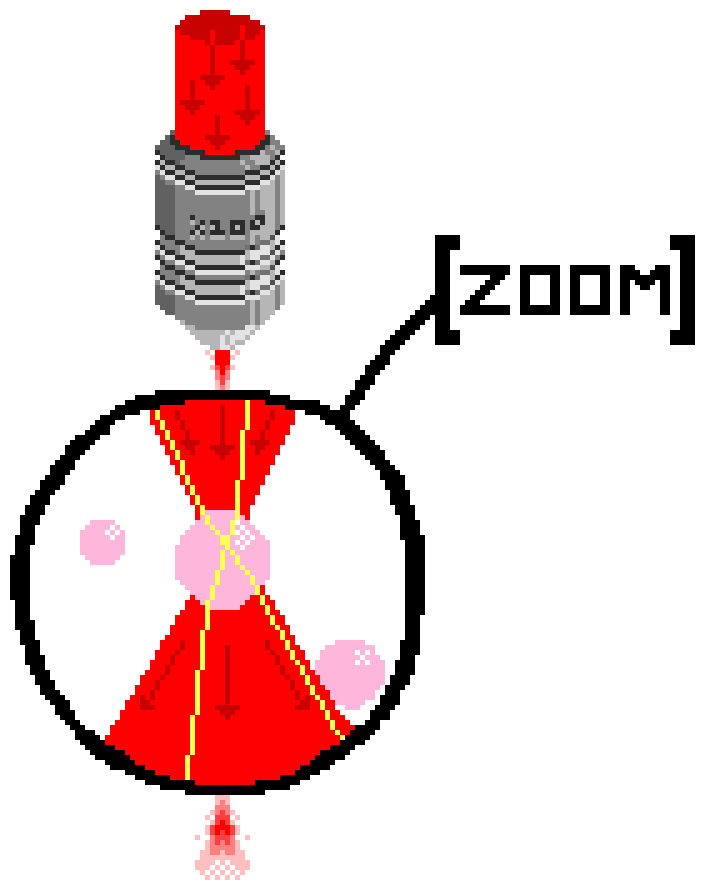
\includegraphics[width=0.5\linewidth,angle=0]{./figures/lazor_zoom}
	\caption{The laser is focused on one point, a particle that gets some rays through it refracts them, and momentum conservation conduct them to be attracted to a point near the focus point.} \label{fig:theory}
	\end{center}
\end{figure}

\section{Dispositif}
There are two main parts to build an optical tweezer:
\begin{itemize}
	\item Microscope
	\item Laser system
\end{itemize}

\subsection{Microscope}
It is made of an objective and an ocular lens. A lamp enlights the sample placed in the focal plane of the objective lens which enlarged the observed object. A shortpass filter that reflects only one kind of electromagnetic wave (one wavelength) is used as a filter : it is placed between the objective and the lens to filter out the laser beam reflected from the sample plate by reflecting it back on the plate. Finally, the ocular lens focus the objective image into the CCD camera which shows us the image on a monitor screen. Experimentally, it has been constated that the last lens had no really other effects than making the final image bigger or smaller.

\subsection{Laser system}
The laser is sent into the microscope objective using some mirrors and a dichoirc mirror. It reflects the laser beam on one direction and let it pass on the other direction.
Initially, the laser is colimated, but since it is too small one should enlarged it, using 2 lens placed in each other focal plane, thus to create a telescope. Therefore, the laser is enlarged and slightly diverging when arriving into the objective. This particular configuration helps to the trapping force effect.

\begin{figure}[h]
	\begin{center}
		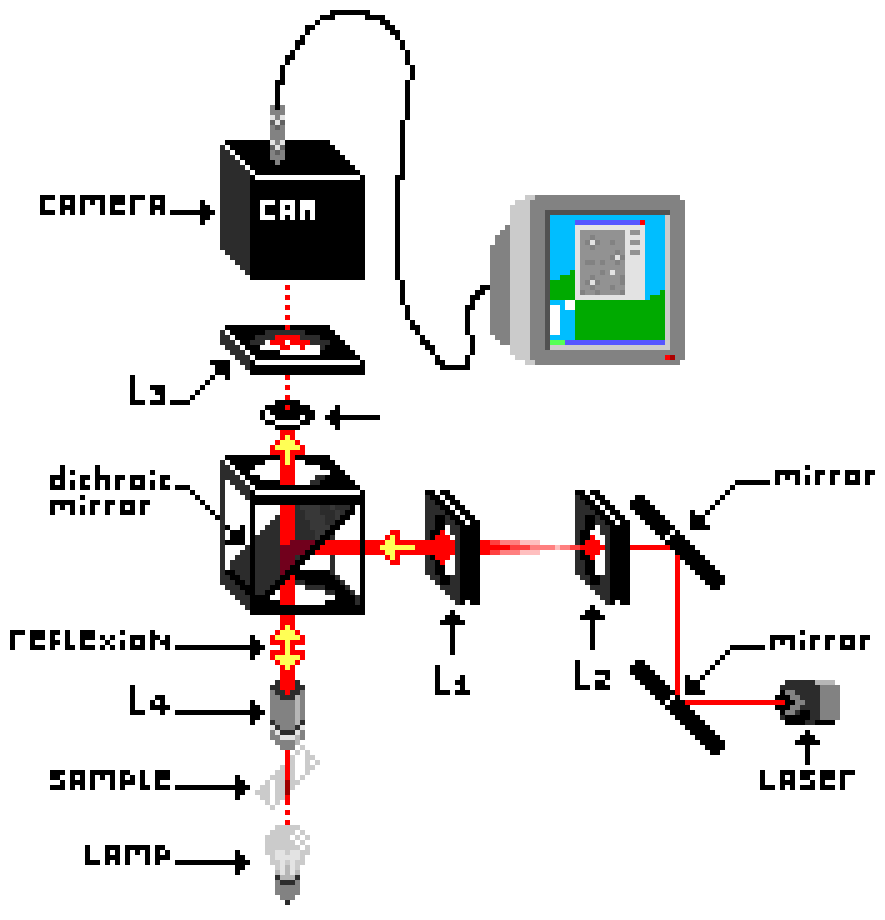
\includegraphics[width=0.8\linewidth,angle=0]{./figures/montage_1}
		\caption{Optical tweezer setup schema.} \label{fig:dispositif}
	\end{center}
\end{figure}

\section{Results}
\subsection{Calibration}
The first task is to calibrate the microscope using a resolution test target (R3L3S1P - Positive 1951 USAF), the results are reasumed in the table~\ref{tab:calibration}

\begin{table}[h!]
\centering
	\begin{tabular}{|c|c|c|c|}
		\hline
		schema & lines pair by milliter[$LP/mm$]& pixel by lines[$Pixel/L$] & [$mm/Pixel$]\\
		\hline
		7.1	& 128.0	& 52 & 7.51e-05\\
		7.2	& 144.0	& 46 & 7.54e-05\\
		7.3	& 161.0	& 41 & 7.57e-05\\
		7.5	& 203.0	& 33 & 7.46e-05\\
		7.6	& 228.0	& 30 & 7.30e-05\\
		\hline
	\end{tabular}
	\caption{Calibration values table}
	\label{tab:calibration}
\end{table}

The microscope part did work well. After many observations on serval samples with different concentrations, it was possible to get a $4000 $x zoom with a clear image when the focus was correct. All particles were distinguishable and it was observed that if a partcle moved on z, the focus was easly lost but that did happen slowly, so it was not a big problem to collect data. It had been a delicate task to find the best lighting so that the algorithm of the given software (MOSAIC in imageJ) can detect some particles (the particle had to appear darker or brighter than everything else, the ring shape was not the optimal input).


The trapping part was an other story. The installation worked well in a particular case that did not look like the description in the theory. When the lens were choosed so that they fit the specifications (get a bigger beam with a colimated light beam), the force applied on the particles was weak, almost negligeable. It was hard to catch and move a particle in space. However, when a complety wrong lens was used (L2 had a way too large focal length), there was an other effect and the laser did catch successfully on x and y. There was a very strong force and it was possile to catch a lot of particles in same time, it was possible to see some particles "fall" from a high z to the focal point (a blurry effect made that easy to intuite). With a small sheet of paper, it was possible to see how the laser looked like in the line between L4 and the dichroic mirror : it was almost parallel and slightly growing when approaching the L4 lens. It was seen that the force was much stronger than in the normal case, but there was a problem : the trapping was working only on x and y, not on z, more details about that is given in the next section. The wrong lens was initially choosen by mistake because all lenses were not put in their correct box. Since it had been constated that there were some better results with those wrong lenses, it had been tried some other configurations of pairs of lenses, in some cases with some random lenses and in some cases with a pair that did fit the specification. It had been seen that the best result was always been got by using a lens L2 with a very high focal length, but that the force with the "correct" pair of lens had somme poor attraction (hard to test on x,y and so on z too). 






% ILLUSTRATION DETECTION PARTICULE RING -> GROS CACA

% ILLUSTRATION DETECTION PARTICULE POINT -> TRAJECTOIRE


\begin{table}
	\begin{tabular}{ r|c|c|c| }
		\multicolumn{1}{r}{} &  \multicolumn{1}{c}{Small [$\O 0.5\mu m$]} & 			\multicolumn{1}{c}{Medium [$\O 1.25\mu m$]} & 			\multicolumn{1}{c}{Big [$\O 2.25\mu m$]}\\
		\cline{2-4}						& 1 & 2 & 3 \\
		  								& 1 & 2 & 3 \\

		\cline{2-4} Mean $[m^2/s] \Rightarrow$ & 1 & 2 & 3\\
		\cline{2-4} Theory $[m^2/s] \Rightarrow$ & 4.29e-13 & 1.71e-13 & 9.53e-14\\
		\cline{2-4}
	\end{tabular}
	\caption{Table of the Experimental and Theorical values for the diffusion coefficient.}
	\label{tab:diffusion}
\end{table}

\section{Analysis and Discussion}

By moving the focus, it was possible to see that particles were trapped when the focus was close the bottom plate : it looked that all particles were trapped in a cone under the focal point. When the focus was near the plate, it was possible to see a clear reflexion of the laser in the plate when the filter was removed, and it was on that moment that the force was at the highest point.  

% - expliquer les calculs

% - le trap selon x y : montrer que ca marche

% - le trap selon z : expliquer

% le plus important!!!

\section{Conclusion}

un bref résumé de la manipulation, revenir sur les buts, une analyse avec plus de recul de l'expérience et ses résultats

description du but du TP

description du dispositif experimental

Résumé (abstract)
Introduction (et background théorique)
Dispositif
Résultats
Bibliographie





\end{document} %%%% THE END %%%%


